\documentclass[12pt]{article}
 
\usepackage[margin=1in]{geometry} 
\usepackage{amsmath,amsthm,amssymb, mathtools}
\usepackage{multicol}
\usepackage[subnum]{cases}
\usepackage{relsize}
\usepackage[makeroom]{cancel}
\usepackage[english]{babel}
\usepackage{graphicx}
\usepackage{calligra}
\usepackage[normalem]{ulem}
\usepackage{caption}
\usepackage{subcaption}
\usepackage{siunitx}
\usepackage{ mathrsfs }
\usepackage{float}
\usepackage{hyperref}
\usepackage{url}


\DeclareMathAlphabet{\mathcalligra}{T1}{calligra}{m}{n} 
\DeclareFontShape{T1}{calligra}{m}{n}{<->s*[2.2]callig15}{}


% Makes '\sr' make a script r
\newcommand{\sr}{\ensuremath{\mathcalligra{r}}}
 
\newcommand{\N}{\mathbb{N}}
\newcommand{\Z}{\mathbb{Z}}
\newcommand{\ihat}{\boldsymbol{\hat{\textbf{\i}}}}
\newcommand{\jhat}{\boldsymbol{\hat{\textbf{\j}}}}
\newcommand{\khat}{\boldsymbol{\hat{\textbf{k}}}}
\newcommand{\rhat}{\boldsymbol{\hat{\textbf{r}}}}
\newcommand{\srhat}{\boldsymbol{\hat{\textbf{\sr}}}}
\newcommand{\xhat}{\boldsymbol{\hat{\textbf{x}}}}
\newcommand{\yhat}{\boldsymbol{\hat{\textbf{y}}}}
\newcommand{\zhat}{\boldsymbol{\hat{\textbf{z}}}}
\newcommand{\phihat}{\boldsymbol{\hat{\textbf{$\phi$}}}}

\newcommand{\vect}[1]{\boldsymbol{\vec{#1}}}
\newcommand{\fracl}[2]{\mathlarger{\frac{#1}{#2}}}
\newcommand{\dd}{\, \mathrm{d}}
\newcommand{\eo}{\epsilon_\circ}
\newcommand{\mo}{\mu_\circ}
\newcommand{\tder}[2]{\frac{\dd #1}{\dd #2}}
\newcommand{\pder}[2]{\frac{\partial #1}{\partial #2}}
\newcommand{\dtder}[2]{\frac{\dd^2 #1}{\dd #2^2}}
\newcommand{\dpder}[2]{\frac{\partial^2 #1}{\partial #2^2}}
\newcommand{\intas}{ \int_{-\infty}^\infty}
\newcommand{\npar}{\\ \\ \noindent}


\begin{document}

\title{Engineering and Computational Techniques of Particle Detection Utilized in the Compact Muon Solenoid}
\author{Roy Smart \\ Montana State University \\PHSX 451 Elementary Particle Physics}
\maketitle

\section{Introduction}
On July 4th 2012, CERN hosted a press conference to announce their findings from the Large Hadron Collider (LHC) \cite{website:higgs_press}. While the world waited with baited breath, CERN researchers confirmed they had identified a particle with mass 125 GeV \cite{new_higgs}. This discovery implied the existence of the Higgs boson, a particle that has been postulated to exist for at least 60 years \cite{higgs_predict}. 
\npar
The LHC utilizes two complementary general-purpose detectors: ATLAS (A Toroidal LHC ApparatuS) and CMS (Compact Muon Solenoid). The two detectors work independently of one another, and in the case of the Higgs particle, provide independent verification of discovery \cite{lhc_combo}. In this paper, we will explore the engineering strategies of the CMS detector that enabled this unique discovery, and the computational techniques used to validate the existence of the Higgs.


\section{CMS Collaboration Results}
\subsection{Interpreting CMS Data}
The existence of the Higgs boson can not be detected directly, rather it is identified through its decay products \cite{higgs_search}. These decay products are not only produced in the Higgs decay, but are created through the decay of other particles. The decay products produced in reactions of previously discovered particles are known as the ``background'' and the search for the Higgs must show that the rates of the pertinent decays are significantly higher than the background rates of decay.
\npar
The CMS collaboration selected five of the most sensitive decay modes in the low-mass region ($m_H = 110-160 \; \text{GeV}$, where $m_H$ is the invariant mass of the Higgs boson) their search for the Higgs. Two decay modes provided high mass resolution: $H\rightarrow \gamma \gamma$ and $H \rightarrow ZZ \rightarrow 4\ell$; while three other modes only provided low mass resolution: $H \rightarrow WW \rightarrow 2\ell2\nu$; $H \rightarrow \tau \tau$; and $H \rightarrow bb$. The $ZZ$ and $\gamma \gamma$ modes are important because they provide a excellent resolution (1-2 GeV) of the invariant mass of the decay products, and consequently give the best estimate for the value of the Higgs' mass \cite{new_higgs}. In this paper, we will be exploring the CMS collaboration's analysis of the $H \to ZZ$ decay mode, and specific technical information as to how their result was calculated.
\subsection{The $H \to ZZ$ Decay Mode}
The Higgs has two fully leptonic decay modes
\begin{align}
 &H \to WW \to \ell^+\nu \; \ell^- \; \overline{\nu}
\intertext{and}
&H \to ZZ \to \ell^+ \ell^- \ell^+ \ell^- \label{golden}
\intertext{where}
& \ell = [e \; (\text{electron}), \; \mu \; (\text{muon})] \quad \text{and} \quad \nu = (\text{neutrino}) \nonumber
\end{align}
The decay mode (\ref{golden}) is known as the `golden' channel for discovery.  This is due to the fact that the entire decay chain can be fully reconstructed with high resolution \cite{higgs_hunt} because the invariant mass of the electron and muon decay products are easily resolved by the CMS detector \cite{golden_higgs}. The high resolution of the golden channel compared to other decay modes comes with a price: the branching ratio of the $ Z \to \ell^+ \ell^- $ is only 3.37\%, so only 0.5\% of the Higgs bosons which decay via the $ZZ$ channel will decay further into the golden channel\cite{higgs_hunt}. Furthermore, the background signals from quark-antiquark and gluon-gluon processes produce topologically similar events, obscuring possible Higgs detections \cite{new_higgs}.

\begin{figure}[h!]
\centering
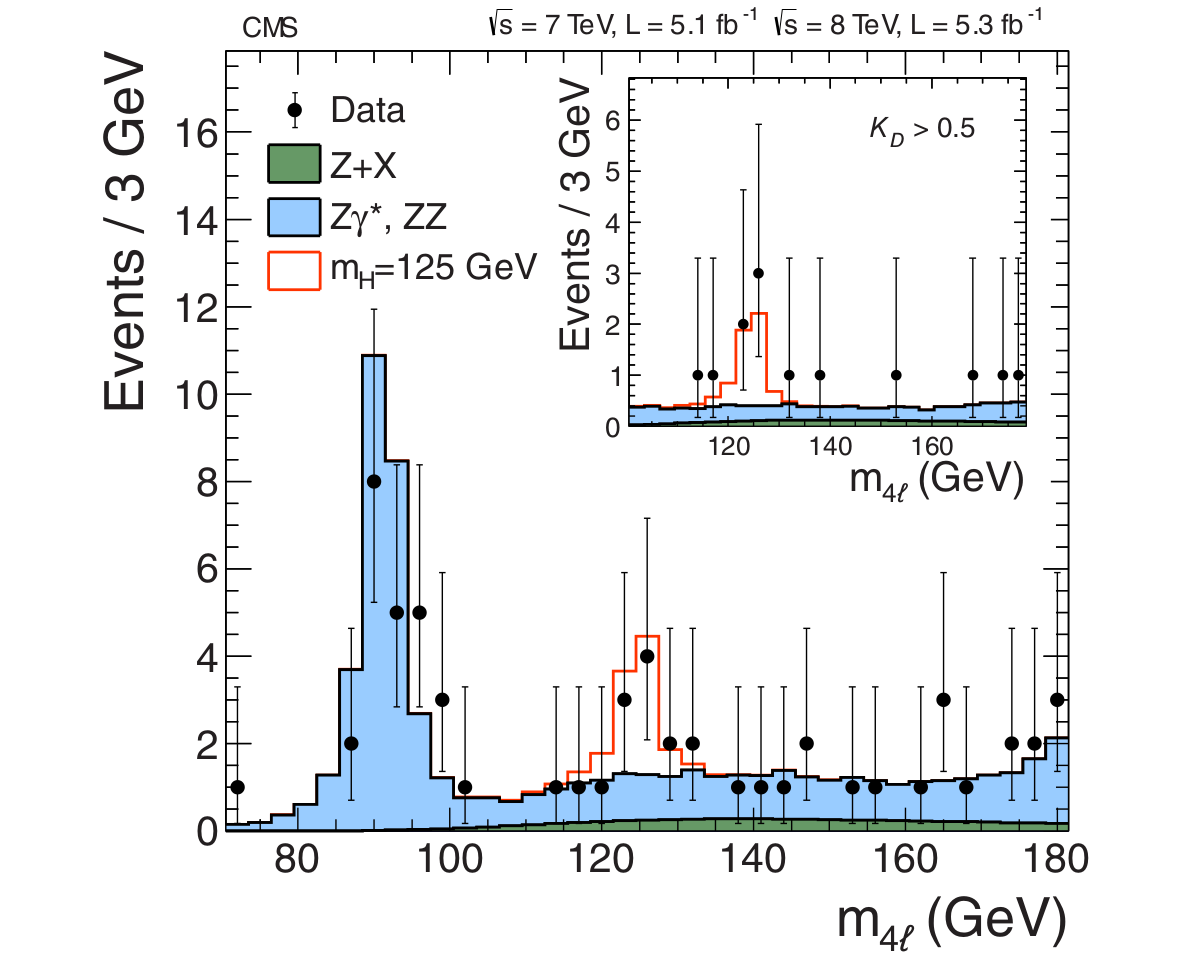
\includegraphics[width=0.8\textwidth]{images/HtoZZ}
\caption{Distribution depicting the four-lepton invariant mass for the CMS collaboration's $ZZ \to 4 \ell$ analysis. The points represent data gathered by the CMS experiment, the filled histograms represent the predicted four-lepton background signal, and the red histogram represents the predicted four-lepton signal for the Higgs boson with a mass of 125 GeV. The inset distribution represents the same plot after the background events have been minimized.}
\label{HtoZZ}
\end{figure}

A graph depicting the evidence of a Higgs boson with a mass of 125 GeV via the $ZZ$ channel is shown in Figure \ref{HtoZZ}. The CMS collaboration utilizes several techniques to minimize the contribution of the background signals. Other than the irreducible quark-antiquark and gluon-gluon processes, there are several background signals that can be minimized:
\begin{align}
& Z + b \overline{b}, \\
& Z + t \overline{t}, \\
& Z + \text{jets}, \qquad \text{and}\\
& WZ + \text{jets} \cite{new_higgs}.
\end{align}
the strategies for eliminating these background processes will be further discussed in Section \ref*{comp_tech}.
\npar
The kinematics of the $H \to ZZ \to 4 \ell$ system can be solved completely in the rest frame of the Higgs using only seven parameters: the invariant masses of the lepton pairs and five angles \cite{new_higgs}, known as Cabibbo-Maksymowicz angles\cite{higgs_angles}. These angles are defined in Table \ref{angle_table} and Figure \ref{angle_fig}. 
\begin{table}[H]
\centering
\begin{tabular}{|c|l|}
\hline
Angle & Description \\ \hline \hline
$\Theta$ & The polar angle of the initial-state partons in the H rest frame. \\ & Measured from the positive z axis (along the anti-clockwise beam direction) \\ \hline
$\theta_1$ & The polar decay angle of the $\ell_1^-$ in the $Z_1$ rest frame. \\ \hline
$\phi_1$ & The azimuthal decay angle of the $\ell_1^-$ in the $Z_1$ rest frame. \\ \hline  
$\theta_2$ & The polar decay angle of the $\ell_2^-$ in the $Z_2$ rest frame. \\ \hline
$\phi_2$ &  The azimuthal decay angle of the $\ell_2^-$ in the $Z_2$ rest frame. \\ \hline
\end{tabular}
\caption{The five Cabibbo-Maksymowicz angles in the $H \to ZZ$ decay mode, and their definitions \cite{higgs_angles}.}
\label{angle_table}
\end{table}

\begin{figure}[h!]
\centering
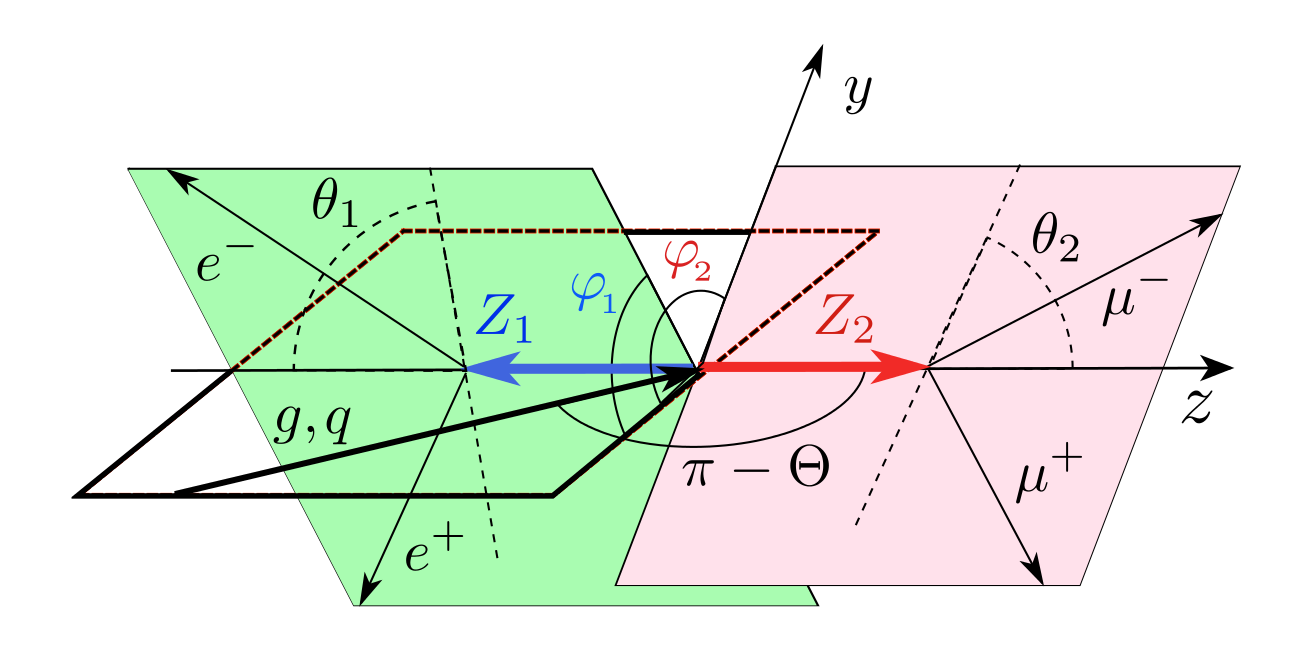
\includegraphics[width=0.8\textwidth]{images/HtoZZ_angles}
\caption{Visual description of the Cabibbo-Maksymowicz angles in the $H \to ZZ$ decay mode \cite{higgs_angles}.}
\label{angle_fig}
\end{figure}
\noindent
We now have an understanding of the parameters associated with identifying the Higgs boson via the $H \to ZZ \to 4 \ell$ decay mode. Next we will explore the design of the CMS experiment and identify what techniques are used to capture this data.

\section{Design of the Compact Muon Solenoid}

\begin{figure}[H]
\centering
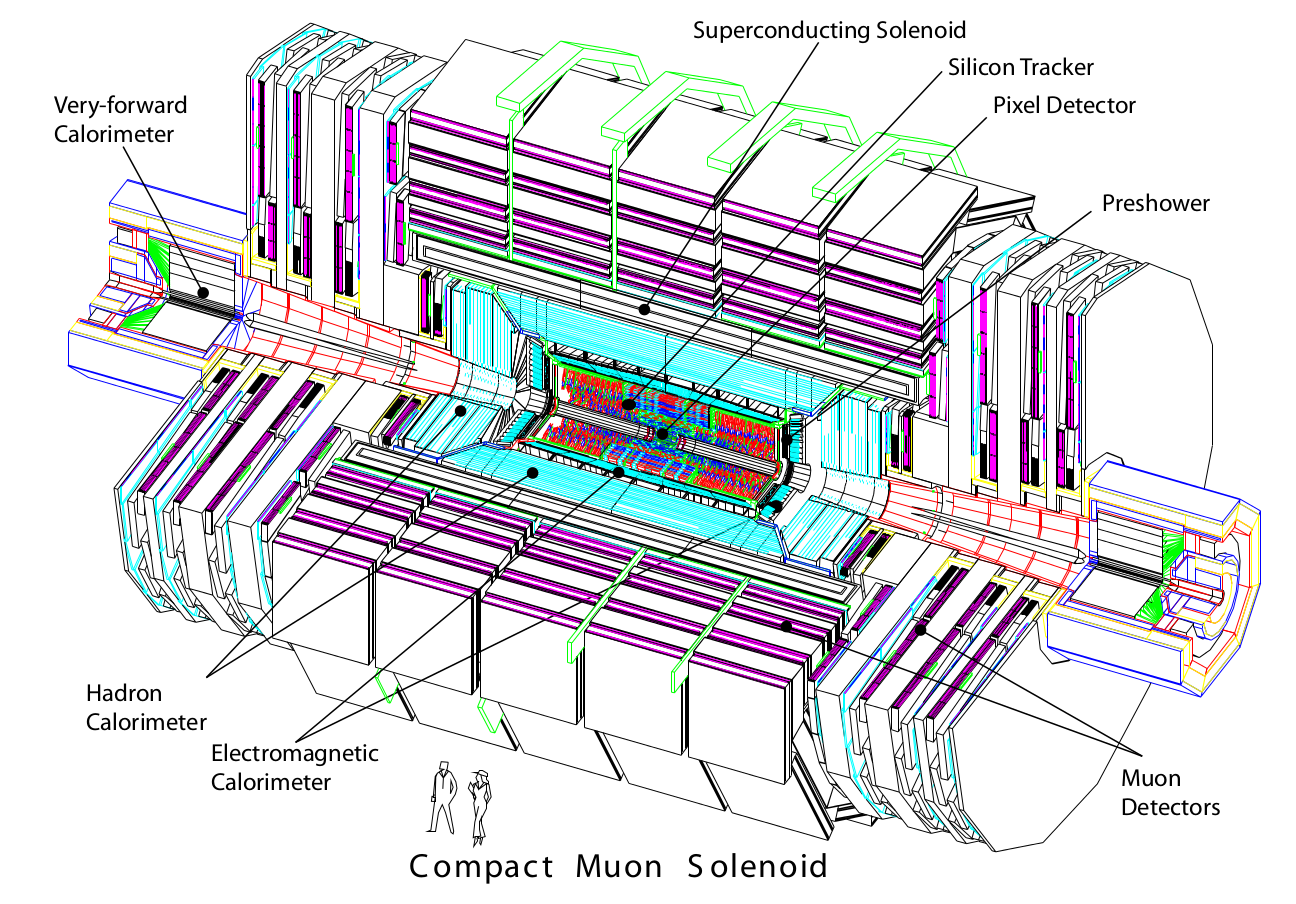
\includegraphics[width = 0.9\textwidth]{images/cms_persp}
\caption{A cut-away perspective view of the CMS experiment, with each of the major sensors within the experiment identified \cite{cms_design}.}
\label{cms_persp}
\end{figure}

\subsection{Overview}
The CMS experiment is designed to identify approximately 1000 charged particles emerging from the interaction region every 25ns. To ensure that the products of a single interaction are interpreted separately and that two subsequent interaction events don't get confused with one another, the experiment must use high-granularity detectors with good time resolution. This results in a large number of detector channels with very low occupancy, which produce an unprecedented amount of data. With these challenges in mind, the requirements of the experiment are as follows:
\begin{itemize}
\item Good muon identification and momentum resolution, with the ability to determine the charge of the muon.
\item Good charged-particle momentum resolution.
\item Good electromagnetic energy resolution, with the ability to isolate photons and leptons.
\item Good missing-transverse-energy and dijet-mass resolution.
\end{itemize}
\noindent
To fulfill these requirements


\section{Computational Techniques}
\label{comp_tech}
\section{Conclusion}



\bibliographystyle{unsrt}
\bibliography{sources}

\section{Questions for first draft}
\begin{enumerate}
\item Should the sources be organized in the order they were cited, or by author's last name?
\item In this paper, particles are identified in italics because \LaTeX \; automatically italicizes characters in math mode. Is this standard notation, or should I make an effort to unitalicize particle symbols?
\item I feel as if I am following the CMS collaborations paper, "Observation of a New Boson at a Mass of 125 Gev with the CMS Experiment at the LHC" too closely, as I have to cite it often. Is this inappropriate for this assignment? Is there a slight modification I can make to my topic to ensure that I don't just restate the work of the CMS collaboration, or is such a situation unavoidable when doing a research paper such as this?
 
\end{enumerate}

\end{document}